\documentclass[conference,10pt]{IEEEtran}

\usepackage[ansinew]{inputenc}
\usepackage[T1]{fontenc}
\usepackage{amsmath}
\usepackage{amssymb}
%\usepackage{graphicx}
\usepackage{float}
\usepackage{cite}
%\usepackage{epsfig,psfrag}
\usepackage{subfigure}
\usepackage{yfonts}
\usepackage{psfrag}


\newtheorem{theorem}{Theorem}
\newtheorem{corollary}{Corollary}

\newcommand{\eref}[1]{(\ref{#1})}
\newcommand{\fref}[1]{Fig.~\ref{#1}}



\def\rec{\rm rec}
\def\inv{\rm inv}
\def\iDC{$i_{\rm DC}$}
\def\rot{A}

\def\rmL{\ell}
\def\rmC{{\rm c} }
\def\rmd{\rm d}
\def\rmo{\rm o}
\def\rmp{\rm p}
\def\rms{\rm s}
\def\Ts{ T_{\rm s}}
\def\Np{ N_{\rm p}}
\def\rmDC{ {\rm dc}}

\def\mA{\mathcal{A}}
\def\mB{\mathcal{B}}
\def\mC{\mathcal{C}}
\def\mD{\mathcal{D}}
\def\mF{\mathcal{F}}
\def\mI{\mathcal{I}}
\def\mL{\mathcal{L}}
\def\mM{\mathcal{M}}
\def\mQ{\mathcal{Q}}
\def\mR{\mathcal{R}}
\def\mU{\mathcal{U}}
\def\mV{\mathcal{V}}
\def\mW{\mathcal{W}}
\def\mX{\mathcal{X}}

\newlength{\mybox}
\setlength{\mybox}{3.8cm}
\newcommand{\vect}[1]{\boldsymbol{#1}}
\newcommand{\mat}[1]{\boldsymbol{#1}}
\newcommand{\legendevert}[1]{\rotatebox{90}{\fbox{\parbox{\mybox}{\centering #1}}}}
\renewcommand{\legendevert}[1]{\rotatebox{90}{{\parbox{\mybox}{\centering #1}}}}
\newlength{\myraiseh}
\newcommand{\unitvert}[1]{\raisebox{\myraiseh}{\legendevert{\footnotesize{#1}}}}
\def\refframe{{f}}
\def\rotorrefframe{{r}}
\def\statorrefframe{{s}}
\newcommand{\rotor}{^{r}}
\newcommand{\stator}{^{s}}

\newcommand{\tb}[1]{\textcolor{red}{TB: #1}}


\bibliographystyle{unsrt}



%
\ifCLASSINFOpdf

v\else

\fi
% epslatex.pdf at: http://www.ctan.org/tex-archive/info/



% correct bad hyphenation here
\hyphenation{op-tical net-works semi-conduc-tor}


\usepackage{color}	% required for `\textcolor' (yatex added)
\usepackage[dvipdfmx]{graphicx}
\graphicspath{{./fig/}}
\begin{document}
%
% paper title
% can use linebreaks \\ within to get better formatting as desired


\title{Model Based Optimal Tuning of Proportional Resonant Controllers}


% author names and affiliations
% use a multiple column layout for up to three different
% affiliations

\author{\IEEEauthorblockN{Topic number: 5}
\IEEEauthorblockA{  }
\IEEEauthorblockE{}}
% author names go here

% conference papers do not typically use \thanks and this command
% is locked out in conference mode. If really needed, such as for
% the acknowledgment of grants, issue a \IEEEoverridecommandlockouts
% after \documentclass

% for over three affiliations, or if they all won't fit within the width
% of the page, use this alternative format:
%
%\author{\IEEEauthorblockN{Michael Shell\IEEEauthorrefmark{1},
%Homer Simpson\IEEEauthorrefmark{2},
%James Kirk\IEEEauthorrefmark{3},
%Montgomery Scott\IEEEauthorrefmark{3} and
%Eldon Tyrell\IEEEauthorrefmark{4}}
%\IEEEauthorblockA{\IEEEauthorrefmark{1}School of Electrical and Computer Engineering\\
%Georgia Institute of Technology,
%Atlanta, Georgia 30332--0250\\ Email: see http://www.michaelshell.org/contact.html}
%\IEEEauthorblockA{\IEEEauthorrefmark{2}Twentieth Century Fox, Springfield, USA\\
%Email: homer@thesimpsons.com}
%\IEEEauthorblockA{\IEEEauthorrefmark{3}Starfleet Academy, San Francisco, California 96678-2391\\
%Telephone: (800) 555--1212, Fax: (888) 555--1212}
%\IEEEauthorblockA{\IEEEauthorrefmark{4}Tyrell Inc., 123 Replicant Street, Los Angeles, California 90210--4321}}



\maketitle


\begin{abstract}
The paper considers the optimal choice of gains of proportional-resonant controllers. A converter, controlled in closed loop, but without proportional resonant controllers, is modeled as a second order transfer function from reference to output. The system is augmented by proportional-resonant control by feeding the error between reference and output back through a set of $N$ proportional resonant controller to subsequently alter the reference. The root locus of the closed loop system is considered as a function of the proportional-resonant gains. To find the optimal choice of gains, we maximize the damping of the mode with smallest damping. This corresponds to solving a nonlinear min-max problem. After linearization, the problem is stated as a linear program.
\end{abstract}





\IEEEpeerreviewmaketitle


\section{Introduction}
Uninterruptible power source (UPS) systems are used in industrial processes in order to decouple loads partially from the grid. Short power outages are compensated and the load is supplied with a clean voltage waveform. Furthermore, UPS systems mitigate the injection of current harmonics to the utility grid that originate from high power non-linear loads.  Consequently, converters for UPS applications are required to have a very high output voltage quality even in presence of highly non-linear loads such as diode rectifiers.

The system efficiency is a key aspect of such systems. Usually, very low semiconductor switching frequencies in the range of 2-4 kHz are employed in order to limit the switching losses and keep the efficiency high. Passive filter components such as inductors and capacitors are minimized such that further power losses are avoided. The filtering performance of these passive filters is usually poor for low order harmonics of non-linear loads. Therefore, the output voltage quality has to be ensured by means of proper control.

Due to the low switching frequency, the closed loop voltage control bandwidth is limited and usually not sufficient to cope with non-linear loads. Additional means of compensating the voltage harmonics are required such as harmonic compensators tuned at the specific harmonic frequencies. Harmonic compensators can be implemented e.g. with proportional resonant (PR) controllers suggested in \cite{924769,4270758,6408064,6153368,993175,5398914,989372}.

Although the performance of proportional resonant controllers in compensating harmonics was investigated extensively, only few publications deal with the proper selection and tuning of the gains of the PR controllers. \cite{5338054} and \cite{6870109} provide analytical parameter tuning rules, but only for a system with single PR controllers tuned at the fundamental frequency. For systems containing several PR controllers tuned at the harmonic frequencies, approximate and empiric parameter tuning rules are given in \cite{924769} and \cite{6153368}. In \cite{5398914}, it is suggested to investigate the bode-plot of the open loop transfer function and design for phase margin. However, this approach should only be applied to closed-loop systems that can be represented as a second order system. Due to the introduction of the harmonic compensators, additional poles are introduced and the system is turned into a high order system. Designing for phase margin can lead to unexpected closed loop system behavior in that case.

Summarizing, no systematic parameter tuning approach considering the interactions of the individual PR controllers and the impact on the damping of the resonant modes is given.

In this paper, a method is presented to optimally choose the gains of the PR controllers. The root locus of the closed loop system is considered as a function of the proportional-resonant gains. To find the optimal choice of gains, we consider maximizing the damping of the mode with smallest damping. This corresponds to solving a nonlinear min-max problem. After linearization, the problem is stated as a linear program which can be solved efficiently.






\section{Converter Model}

%-----------------------------------------
%\begin{figure}[!h]
%\centering
%\input{fig/VoltageSourceInverter.pstex_t}
%\caption{Voltage source inverter connecting a DC link capacitance with an output LC filter.}
%\label{fig:VoltageSourceInverter}
%\end{figure}
%-----------------------------------------

Our starting point is to consider a voltage source inverter (VSI) which is assumed to operate in closed loop, but without PR controllers.  The controlled inverter is modeled as a second order transfer function which maps the (sinusoidal) reference to the output,
\begin{align}
\label{eq:InvMdl}
y = G(s)y_{\rm ref},\quad G(s) = \frac{\omega^2}{s^2+\xi\omega s + \omega^2}\,,
\end{align}
where $\omega$ is the natural frequency and $\xi$ is the damping of the controlled inverter. One example of a system which can be modeled as such,
is a VSI with LC filter, %as the one shown in Figure~\ref{fig:VoltageSourceInverter},
controlled in abc frame by a cascaded voltage-current control system comprising proportional controllers.
We note that, with properly designed control, a VSI is expected to behave as second order systems in closed loop. Thus, assuming a system model of the form~(\ref{eq:InvMdl}) is not restrictive.

%The output voltage of voltage source inverters is generated by a frequent switching between different voltage levels on the DC side. The generated voltages can thus be described as piecewise constant voltages; the output voltage is finally obtained by low-pass filtering the piecewise constant voltage by means of LC circuits. The output voltage contains not only the requested reference voltage, but also harmonics.


\subsection{Proportional-resonant controllers}

To achieve offset free tracking of the sinusoidal reference $y_{\rm ref}$ and to reduce harmonics in the output, we consider adding PR controllers~\cite{fukuda2001novel} to the system~(\ref{eq:InvMdl}).
The PR controllers are added in an outer loop (see Fig.~\ref{fig:ControlStructure}) and adjust the reference according to
\begin{align*}
\tilde{y}_{\rm ref} = y_{\rm ref} + \sum_{n\in\{1,3,5,\dots, N\}}H_n(s)(y_{\rm ref}-y)\,,
\end{align*}
where
\begin{align*}
H_n(s) = \frac{\lambda_ns}{s^2 + (n\omega_0)^2}\,,
\end{align*}
where the fundamental frequency $\omega_0$ is the frequency of the reference (typically 50 or 60 Hz), and where $\lambda_n$ are the feedback gains of the PR controllers. These gains are tuning parameters whose value affect the transient response of the closed loop system.
%-----------------------------------------
\begin{figure}[!h]
\centering
\input{fig/ControlStructure.pstex_t}
\caption{Control structure of converter model with PR controllers.}
\label{fig:ControlStructure}
\end{figure}
%-----------------------------------------


\subsection{Closed loop system}

The order of the closed loop system dynamics is $2+2N_{\rm PR}$ where $N_{\rm PR}$ is the number of PR controllers added in the outer loop. The resulting closed-loop system can be stated as
\begin{align}\label{eq:ClosedLoopTF}
  y = \frac{G(s) + G(s) \sum_n H_n(s)}{I + G(s) \sum_n H_n(s)} y_{\rm ref}\,,
\end{align}
and by changing the gains $\lambda_n$, we influence the location of the poles and zeros of the closed-loop system.


\subsection{Closed loop poles}
The PR gains $\lambda_n$ affect both the poles of the closed loop system. In the design approach outlined below, we seek to maximize the damping of the (complex) pole pair which has the lowest damping.

To clarify the approach we consider an example: Consider the case where two PR controllers (with harmonics number $1$ and $3$) are included in the control loop. For this case the system has $6$ poles, and their position in the complex plane is determined by  two gains $\lambda_1$, $\lambda_3$.
We enumerate different combinations of gains $\lambda_1$, $\lambda_3$ and plot the resulting poles on the complex plane; the result is shown in Fig.~\ref{fig:PoleExample}. In this figure we also plot the poles obtained when both gains are close to zero (blue circles), and the poles obtained with one particular choice of higher gains (red circles).
%The poles obtained with low and high gains are shown by blue and red circles, respectively.

From Fig.~\ref{fig:PoleExample} it can be seen that one pole pair moves to the right, closer to the imaginary axis (and unstable domain), while the other two pole pairs move left. For sufficiently high gains, one of the pole pairs turn into two purely real poles, one of which moves left and the other moves right, towards the unstable domain.
%-----------------------------------------
\begin{figure}[!h]
\centering
% Generated using matlabfrag
% Version: v0.6.16
% Version Date: 04-Apr-2010
% Author: Zebb Prime
%
%% <text>
%
\providecommand\matlabtextA{\color[rgb]{0.000,0.000,0.000}\fontsize{8}{8}\selectfont\strut}%
\psfrag{011}[cl][cl]{\matlabtextA $\alpha_i$}%
%
\providecommand\matlabtextB{\color[rgb]{0.150,0.150,0.150}\fontsize{8}{8}\selectfont\strut}%
\psfrag{012}[tc][tc]{\matlabtextB Real}%
\psfrag{013}[bc][bc]{\matlabtextB Imaginary}%
%
%% </text>
%
%% <xtick>
%
\def\matlabfragNegXTick{\mathord{\makebox[0pt][r]{$-$}}}
%
\psfrag{000}[ct][ct]{\matlabtextB $\matlabfragNegXTick 1500$}%
\psfrag{001}[ct][ct]{\matlabtextB $\matlabfragNegXTick 1000$}%
\psfrag{002}[ct][ct]{\matlabtextB $\matlabfragNegXTick 500$}%
\psfrag{003}[ct][ct]{\matlabtextB $0$}%
%
%% </xtick>
%
%% <ytick>
%
\psfrag{004}[rc][rc]{\matlabtextB $-1500$}%
\psfrag{005}[rc][rc]{\matlabtextB $-1000$}%
\psfrag{006}[rc][rc]{\matlabtextB $-500$}%
\psfrag{007}[rc][rc]{\matlabtextB $0$}%
\psfrag{008}[rc][rc]{\matlabtextB $500$}%
\psfrag{009}[rc][rc]{\matlabtextB $1000$}%
\psfrag{010}[rc][rc]{\matlabtextB $1500$}%
%
%% </ytick>
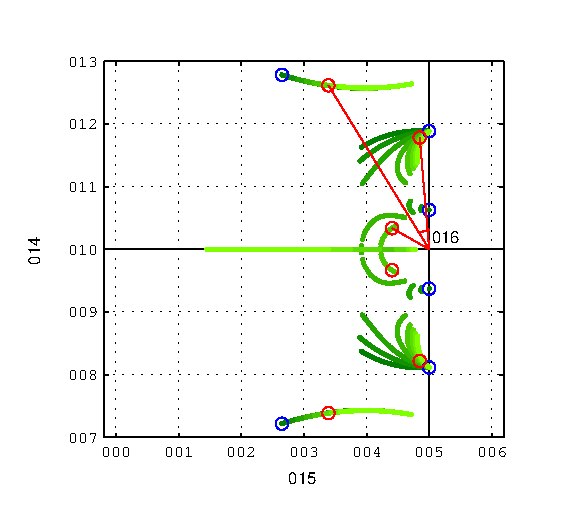
\includegraphics{fig/root_locus_2D}
\caption{Poles of the closed loop system with $N_{PR}=2$ PR controllers: The green points show poles for various combinations of gains $\lambda_1$,
$\lambda_3$. Blue circles show the poles for low gains. Red circles show poles for high gains. }
\label{fig:PoleExample}
\end{figure}
%-----------------------------------------

Since changes in one gain affects all poles, it is not obvious how to choose the gains optimally. Increase in one particular gain may make one pole pair ``more stable'', but may have negative effects on another pole pair.






\section{Problem Formulation}
To address the problem of how to choose the PR gains, we propose to formulate a max-min optimization problem, where we maximize the damping of the least damped pole pair. More precisely, we consider the angle between the pole and the imaginary axis (assuming the pole is in the open left half plane);
\begin{align*}
\alpha_i = \tan^{-1}(-{\rm real}(p_i) / {\rm imag}(p_i))
\end{align*}
where $p_i$ is a pole in the fourth quadrant. The problem we ideally want to solve is
\begin{align}
\label{eq:MaxMinProb}
\max_{\lambda_1,\lambda_3,\dots, \lambda_N}\min_{i\in \{1, \dots, i_{\rm max}\}} \alpha_i(\lambda_1,\lambda_3,\dots, \lambda_N).
\end{align}
with $i_{\rm max} = (N+3)/2$. We note that the angles $\alpha_i$ are dependent on the PR gains $\lambda_n$, and that as the gains vary, different angles take on the role of being ``the least damped''.

%For one combination of PR gains, the resulting dampings $\alpha_i$ are indicated in Figure~\ref{fig:PoleExample}.

Figure~\ref{fig:DampingExample} shows $\min_{i\in\{1,2,3\}}\alpha_i$; the smallest damping of the three pole pairs as a function of the gains. High gains for both PR controllers push one pole into the right half plane, resulting in an unstable system.
%-----------------------------------------
\begin{figure}[!h]
\centering
% Generated using matlabfrag
% Version: v0.6.16
% Version Date: 04-Apr-2010
% Author: Zebb Prime
%
%% <text>
%
\providecommand\matlabtextA{\color[rgb]{0.150,0.150,0.150}\fontsize{8}{8}\selectfont\strut}%
\psfrag{013}[tl][tl]{\matlabtextA $\lambda_1$}%
\psfrag{014}[tr][tr]{\matlabtextA $\lambda_3$}%
\psfrag{015}[bc][bc]{\matlabtextA damping [deg]}%
%
%% </text>
%
%% <xtick>
%
\def\matlabfragNegXTick{\mathord{\makebox[0pt][r]{$-$}}}
%
\psfrag{000}[ct][ct]{\matlabtextA $0$}%
\psfrag{001}[ct][ct]{\matlabtextA $500$}%
\psfrag{002}[ct][ct]{\matlabtextA $1000$}%
%
%% </xtick>
%
%% <ytick>
%
\psfrag{003}[rc][rc]{\matlabtextA $0$}%
\psfrag{004}[rc][rc]{\matlabtextA $200$}%
\psfrag{005}[rc][rc]{\matlabtextA $400$}%
\psfrag{006}[rc][rc]{\matlabtextA $600$}%
\psfrag{007}[rc][rc]{\matlabtextA $800$}%
\psfrag{008}[rc][rc]{\matlabtextA $1000$}%
%
%% </ytick>
%
%% <ztick>
%
\psfrag{009}[cr][cr]{\matlabtextA $0$}%
\psfrag{010}[cr][cr]{\matlabtextA $10$}%
\psfrag{011}[cr][cr]{\matlabtextA $20$}%
\psfrag{012}[cr][cr]{\matlabtextA $30$}%
%
%% </ztick>
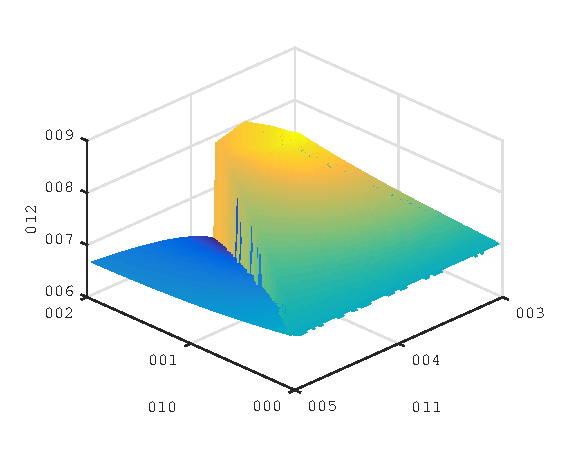
\includegraphics{fig/root_locus_2D_in_3D}
\caption{Minimum of the damping $\alpha_i$ of the pole pairs of the closed loop system with $N_{\rm PR}=2$ PR controllers as a function of the PR controller gains $\lambda_1$ and $\lambda_3$. The labels on the contour lines indicate damping in degrees.}
\label{fig:DampingExample}
\end{figure}
%-----------------------------------------


\subsection{Problem approximation}

To obtain a tractable optimization problem, we proceed to approximate $\alpha_i(\lambda_1,\lambda_3,\dots\lambda_N)$ with affine functions of the gains $\lambda_n$: That is, the angles are approximated by
\begin{align}
\label{eq:AngleApprox}
\tilde{\alpha}_i(\lambda_1,\lambda_3,\dots, \lambda_N)
= a_i^T\lambda + b_i
\end{align}
where
%\begin{align*}
$\lambda =
\begin{bmatrix}
\lambda_1 & \lambda_3 & \dots & \lambda_N
\end{bmatrix}^T$
%\end{align*}
is a vector containing the gains and where $a_i\in\mathbb{R}^{N_{\rm PR}}$, $b_i\in\mathbb{R}$ are constant vectors obtained by sampling the value of the angles
$\alpha_i$ for a number of gain combinations, and performing a least squares fit.

By describing the angles in~(\ref{eq:MaxMinProb})
with the approximation~(\ref{eq:AngleApprox}), we obtain a max-min problem with affine cost function:
\begin{align}
\label{eq:MaxMinProbApprox}
\max_{\lambda_1,\lambda_3,\dots, \lambda_N}\min_{i\in \{1, \dots, i_{\rm max}\}} a_i^T\lambda + b_i.
\end{align}
 This problem can be equivalently formulated a linear program (LP) according to
\begin{align}
\label{eq:MaxMinProbLP}
\min c^Tx,\quad {\rm s.t.} \quad Ax\le b
\end{align}
with matrices
\begin{align*}
A =
\begin{bmatrix}
1 & -c^T_1\\
1 & -c^T_2\\
 & \vdots \\
1 & -c^T_{i_{\rm max}}
\end{bmatrix},\quad
b =
\begin{bmatrix}
b_1\\
b_2\\
\vdots \\
b_{i_{\rm max}}
\end{bmatrix},\quad
c =
\begin{bmatrix}
-1\\
0\\
\vdots \\
0
\end{bmatrix}.
\end{align*}
%{\bf Put derivation in appendix}
Linear programs can be solved efficiently with readily available software.



\section{Numerical Example}

The PR gain optimization was applied to a VSI with LC filter used in UPS applications.
The UPS considered is a four-wire topology where the dynamics of the three phases are decoupled, due to the connection between filter and DC side neutral point. Due to the decoupling, we consider each of the three phases individually and design stabilizing controllers with proportional feedback. The closed loop system thus becomes a second order transfer function from voltage reference to output voltage on the form~(\ref{eq:InvMdl}).
%-----------------------------------------
\begin{figure}[!h]
\centering
\psfrag{vg}{\footnotesize{$i_{\rm load}$}}
\psfrag{x1}{\footnotesize{$i$}}
\psfrag{x3}{\footnotesize{$v$}}
\psfrag{Lfi}{\footnotesize{$L$}}
\psfrag{Cf}{\footnotesize{$C$}}
\psfrag{vdc/2}{\footnotesize{$v_{\rm dc}/2$}}
\psfrag{+}{\tiny{$+$}}
\scalebox{0.9}{
\input{fig/VSC_LC_3ph.pstex_t}
}
%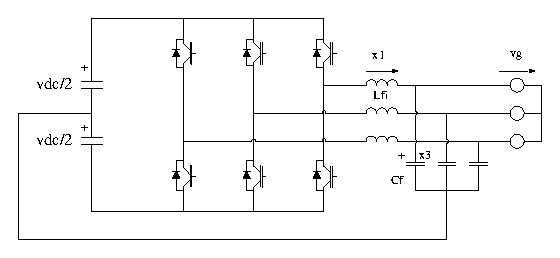
\includegraphics[width=8cm]{fig/VSC_LC_3ph}
\caption{Voltage source inverter with LC filter.}
\label{fig:UPS_LC}
\end{figure}
%-----------------------------------------

The inner control loop is augmented with $N_{\rm PR} = 4$ PR controllers as described in Fig.~\ref{fig:ControlStructure}. We thus have five
angles $\alpha_i$ which are functions of four gains
$\lambda_i$. The nonlinear functions $\alpha_i$ are sampled over a grid of gain values and a linear approximation of the nonlinear functions is made by least squares fitting. The resulting LP~(\ref{eq:MaxMinProbApprox}) is solved. The poles of the system, using the optimal gains, is shown by the red circles in Fig.~\ref{fig:PolesOptimalExample}.
We note that at the optimum, all poles have the same damping and are located on a single line. %in the left half complex plane.
%-----------------------------------------
\begin{figure}[!h]
\centering
% Generated using matlabfrag
% Version: v0.6.16
% Version Date: 04-Apr-2010
% Author: Zebb Prime
%
%% <text>
%
\providecommand\matlabtextA{\color[rgb]{0.150,0.150,0.150}\fontsize{8}{8}\selectfont\strut}%
\psfrag{015}[tc][tc]{\matlabtextA Real Axis}%
\psfrag{016}[bc][bc]{\matlabtextA Imaginary Axis}%
%
%% </text>
%
%% <xtick>
%
\def\matlabfragNegXTick{\mathord{\makebox[0pt][r]{$-$}}}
%
\psfrag{000}[ct][ct]{\matlabtextA $\matlabfragNegXTick 2500$}%
\psfrag{001}[ct][ct]{\matlabtextA $\matlabfragNegXTick 2000$}%
\psfrag{002}[ct][ct]{\matlabtextA $\matlabfragNegXTick 1500$}%
\psfrag{003}[ct][ct]{\matlabtextA $\matlabfragNegXTick 1000$}%
\psfrag{004}[ct][ct]{\matlabtextA $\matlabfragNegXTick 500$}%
\psfrag{005}[ct][ct]{\matlabtextA $0$}%
%
%% </xtick>
%
%% <ytick>
%
\psfrag{006}[rc][rc]{\matlabtextA $-8000$}%
\psfrag{007}[rc][rc]{\matlabtextA $-6000$}%
\psfrag{008}[rc][rc]{\matlabtextA $-4000$}%
\psfrag{009}[rc][rc]{\matlabtextA $-2000$}%
\psfrag{010}[rc][rc]{\matlabtextA $0$}%
\psfrag{011}[rc][rc]{\matlabtextA $2000$}%
\psfrag{012}[rc][rc]{\matlabtextA $4000$}%
\psfrag{013}[rc][rc]{\matlabtextA $6000$}%
\psfrag{014}[rc][rc]{\matlabtextA $8000$}%
%
%% </ytick>
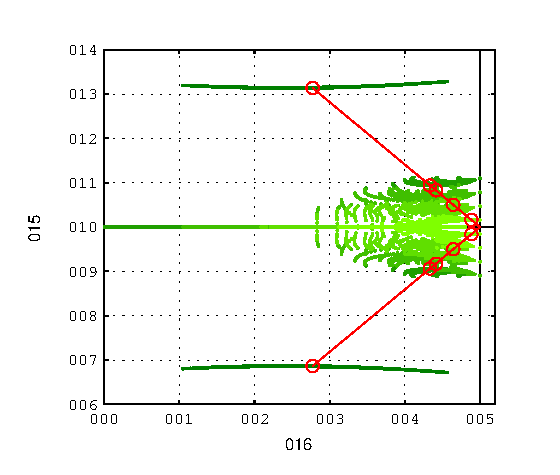
\includegraphics{fig/root_locus}
\caption{Poles of the closed loop system with $N_{PR}=4$ PR controllers: The green points show poles for various combinations of gains $\lambda_1$, $\lambda_3$, $\lambda_5$ and $\lambda_7$. Red circles show poles for the optimal gains.
We note that for the optimal gains, all poles have the same damping and are located on a single line in the left half complex plane.
}
\label{fig:PolesOptimalExample}
\end{figure}
%-----------------------------------------


%\subsection{Simulation}
%\subsection{Transient performance}
The system is simulated with a nonlinear load; a diode rectifier bridge. The dynamic response and the steady state behavior with and without PR controllers is evaluated in simulation. All values are in per unit.

When the system is at steady state the load is switched out. The transient response of the output voltage is shown in Fig.~\ref{fig:trans_vc}. It can be seen that the introduction of the PR controllers (blue line) causes some more extended oscillation, but only a minor increase of the overshoot.
%-----------------------------------------
\begin{figure}[!h]
\centering
% Generated using matlabfrag
% Version: v0.6.16
% Version Date: 04-Apr-2010
% Author: Zebb Prime
%
%% <text>
%
\providecommand\matlabtextA{\color[rgb]{0.000,0.000,0.000}\fontsize{8}{8}\selectfont\strut}%
\psfrag{014}[cl][cl]{\matlabtextA without PRs}%
\psfrag{015}[cl][cl]{\matlabtextA with PRs}%
\psfrag{016}[bc][bc]{\matlabtextA voltage [pu]}%
\psfrag{017}[tc][tc]{\matlabtextA time [s]}%
%
%% </text>
%
%% <xtick>
%
\def\matlabfragNegXTick{\mathord{\makebox[0pt][r]{$-$}}}
%
\psfrag{000}[ct][ct]{\matlabtextA $0.4$}%
\psfrag{001}[ct][ct]{\matlabtextA $0.402$}%
\psfrag{002}[ct][ct]{\matlabtextA $0.404$}%
\psfrag{003}[ct][ct]{\matlabtextA $0.406$}%
\psfrag{004}[ct][ct]{\matlabtextA $0.408$}%
\psfrag{005}[ct][ct]{\matlabtextA $0.41$}%
\psfrag{006}[ct][ct]{\matlabtextA $0.412$}%
%
%% </xtick>
%
%% <ytick>
%
\psfrag{007}[rc][rc]{\matlabtextA $-1.5$}%
\psfrag{008}[rc][rc]{\matlabtextA $-1$}%
\psfrag{009}[rc][rc]{\matlabtextA $-0.5$}%
\psfrag{010}[rc][rc]{\matlabtextA $0$}%
\psfrag{011}[rc][rc]{\matlabtextA $0.5$}%
\psfrag{012}[rc][rc]{\matlabtextA $1$}%
\psfrag{013}[rc][rc]{\matlabtextA $1.5$}%
%
%% </ytick>
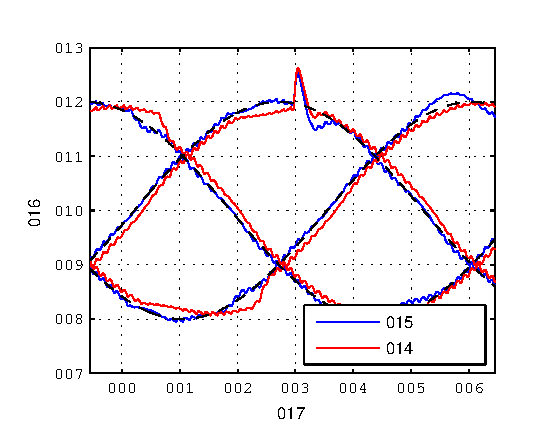
\includegraphics{fig/transient_vCf}
\caption{Transient response of the output voltage when the load (a diode rectifier bridge) is switched out.}
\label{fig:trans_vc}
\end{figure}
%-----------------------------------------

<<<<<<< HEAD
%\subsection{Steady state performance}
The steady state output voltage and load current are shown in Fig.~\ref{fig:ss_vc} and \ref{fig:ss_iload}. The harmonics of the steady state voltage are shown in Fig.~\ref{fig:ss_harm}. From Fig.~\ref{fig:ss_harm}, it can be seen that the PR controllers (blue circles) reduce the third, fifth and seventh harmonics, while some of the higher order harmonics increase.
=======

\subsection{Steady state performance}
The system is simulated with a nonlinear load; we consider a diode rectifier bridge. The steady state output voltage and load current are shown in Fig.~\ref{fig:ss_vc} and \ref{fig:ss_iload}. The harmonics of the steady state voltage are shown in Fig.~\ref{fig:ss_harm}. All values are in per unit.



>>>>>>> 261d4d0f08281c23f0218e1f765cbcd93ee3dee2
%-----------------------------------------
\begin{figure}[!h]
\centering
% Generated using matlabfrag
% Version: v0.6.16
% Version Date: 04-Apr-2010
% Author: Zebb Prime
%
%% <text>
%
\providecommand\matlabtextA{\color[rgb]{0.000,0.000,0.000}\fontsize{8}{8}\selectfont\strut}%
\psfrag{010}[cl][cl]{\matlabtextA c}%
\psfrag{011}[cl][cl]{\matlabtextA b}%
\psfrag{012}[cl][cl]{\matlabtextA a}%
\psfrag{013}[bc][bc]{\matlabtextA phase voltage [V]}%
\psfrag{014}[tc][tc]{\matlabtextA time [s]}%
%
%% </text>
%
%% <xtick>
%
\def\matlabfragNegXTick{\mathord{\makebox[0pt][r]{$-$}}}
%
\psfrag{000}[ct][ct]{\matlabtextA $0$}%
\psfrag{001}[ct][ct]{\matlabtextA $0.005$}%
\psfrag{002}[ct][ct]{\matlabtextA $0.01$}%
\psfrag{003}[ct][ct]{\matlabtextA $0.015$}%
\psfrag{004}[ct][ct]{\matlabtextA $0.02$}%
%
%% </xtick>
%
%% <ytick>
%
\psfrag{005}[rc][rc]{\matlabtextA $-1$}%
\psfrag{006}[rc][rc]{\matlabtextA $-0.5$}%
\psfrag{007}[rc][rc]{\matlabtextA $0$}%
\psfrag{008}[rc][rc]{\matlabtextA $0.5$}%
\psfrag{009}[rc][rc]{\matlabtextA $1$}%
%
%% </ytick>
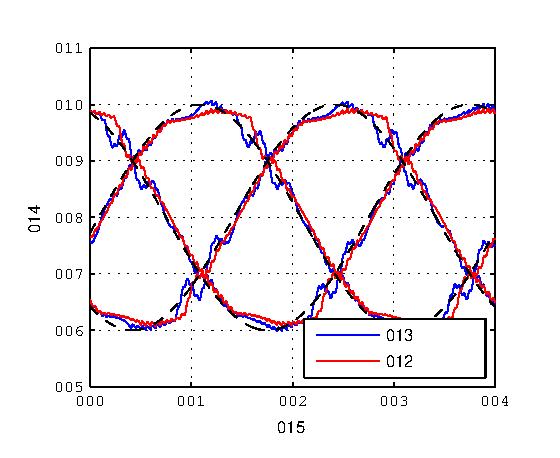
\includegraphics{fig/steady_state_vCf}
\caption{Steady state output voltage with diode rectifier bridge as load.}
\label{fig:ss_vc}
\end{figure}
%-----------------------------------------
%-----------------------------------------
\begin{figure}[!h]
\centering
% Generated using matlabfrag
% Version: v0.6.16
% Version Date: 04-Apr-2010
% Author: Zebb Prime
%
%% <text>
%
\providecommand\matlabtextA{\color[rgb]{0.000,0.000,0.000}\fontsize{8}{8}\selectfont\strut}%
\psfrag{011}[cl][cl]{\matlabtextA c}%
\psfrag{012}[cl][cl]{\matlabtextA b}%
\psfrag{013}[cl][cl]{\matlabtextA a}%
\psfrag{014}[bc][bc]{\matlabtextA phase current [A]}%
\psfrag{015}[tc][tc]{\matlabtextA time [s]}%
%
%% </text>
%
%% <xtick>
%
\def\matlabfragNegXTick{\mathord{\makebox[0pt][r]{$-$}}}
%
\psfrag{000}[ct][ct]{\matlabtextA $0$}%
\psfrag{001}[ct][ct]{\matlabtextA $0.005$}%
\psfrag{002}[ct][ct]{\matlabtextA $0.01$}%
\psfrag{003}[ct][ct]{\matlabtextA $0.015$}%
\psfrag{004}[ct][ct]{\matlabtextA $0.02$}%
%
%% </xtick>
%
%% <ytick>
%
\psfrag{005}[rc][rc]{\matlabtextA $-1.5$}%
\psfrag{006}[rc][rc]{\matlabtextA $-1$}%
\psfrag{007}[rc][rc]{\matlabtextA $-0.5$}%
\psfrag{008}[rc][rc]{\matlabtextA $0$}%
\psfrag{009}[rc][rc]{\matlabtextA $0.5$}%
\psfrag{010}[rc][rc]{\matlabtextA $1$}%
%
%% </ytick>
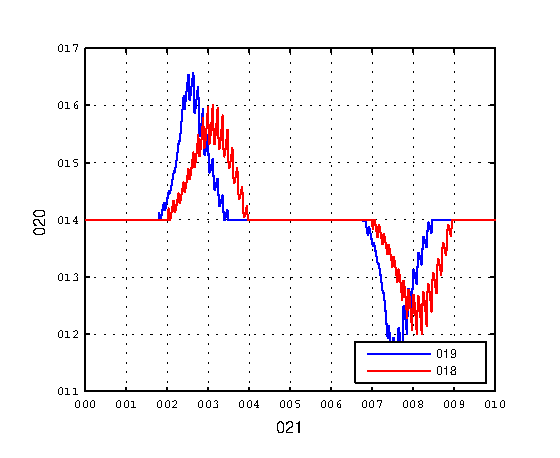
\includegraphics{fig/steady_state_iLoad}
\caption{Steady state load current with diode rectifier bridge as load.}
\label{fig:ss_iload}
\end{figure}
%-----------------------------------------
%-----------------------------------------
\begin{figure}[!h]
\centering
% Generated using matlabfrag
% Version: v0.6.16
% Version Date: 04-Apr-2010
% Author: Zebb Prime
%
%% <text>
%
\providecommand\matlabtextA{\color[rgb]{0.000,0.000,0.000}\fontsize{8}{8}\selectfont\strut}%
\psfrag{014}[cl][cl]{\matlabtextA without PRs}%
\psfrag{015}[cl][cl]{\matlabtextA with PRs}%
\psfrag{016}[bc][bc]{\matlabtextA amplitude [dB]}%
\psfrag{017}[tc][tc]{\matlabtextA harmonic number}%
%
%% </text>
%
%% <xtick>
%
\def\matlabfragNegXTick{\mathord{\makebox[0pt][r]{$-$}}}
%
\psfrag{000}[ct][ct]{\matlabtextA $0$}%
\psfrag{001}[ct][ct]{\matlabtextA $5$}%
\psfrag{002}[ct][ct]{\matlabtextA $10$}%
\psfrag{003}[ct][ct]{\matlabtextA $15$}%
\psfrag{004}[ct][ct]{\matlabtextA $20$}%
\psfrag{005}[ct][ct]{\matlabtextA $25$}%
\psfrag{006}[ct][ct]{\matlabtextA $30$}%
%
%% </xtick>
%
%% <ytick>
%
\psfrag{007}[rc][rc]{\matlabtextA $-60$}%
\psfrag{008}[rc][rc]{\matlabtextA $-50$}%
\psfrag{009}[rc][rc]{\matlabtextA $-40$}%
\psfrag{010}[rc][rc]{\matlabtextA $-30$}%
\psfrag{011}[rc][rc]{\matlabtextA $-20$}%
\psfrag{012}[rc][rc]{\matlabtextA $-10$}%
\psfrag{013}[rc][rc]{\matlabtextA $0$}%
%
%% </ytick>
\includegraphics{fig/steady_state_harmonics}
<<<<<<< HEAD
\caption{Harmonics of he steady state output voltage with diode rectifier bridge as load.}
=======
\caption{Harmonics of the steady state output voltage.}
>>>>>>> 261d4d0f08281c23f0218e1f765cbcd93ee3dee2
\label{fig:ss_harm}
\end{figure}
%-----------------------------------------




\bibliography{IPECrefs}

% that's all folks
\end{document}


